\section{Physikalische Grundlagen}

\subsection{Hyperfeinstruktur und Zeeman-Effekt}
Dieser Abschnitt orientiert sich an \cite{staatsex}. \\
Die \emph{Hyperfeinstrukturaufspaltung} entsteht durch die Wechselwirkung von \emph{Kernspin} $\vec{I}$ und 
\emph{elektronischem Gesamtdrehimpuls} $\vec{J}$. Für den \emph{Gesamtdrehimpuls} $\vec{F}$ des Atoms gilt:
\begin{equation}
    \vec{F} = \vec{I} + \vec{J}, \qquad \abs{I - J} \leq F \leq I + J
\end{equation}
Der Kernspin beschreibt den Drehimpuls des Kerns, mit ihm ist ein magnetisches Moment 
$\vec{\mu}_I = \frac{g_I \mu_K}{\hbar} \vec{I}$ ($g_I$ ist der \emph{Kern-g-Faktor} und
$\mu_K$ das \emph{Kernmagneton}) verbunden. \\
Die Energieaufspaltung $\Delta E_\text{HFS}$ der Hyperfeinstruktur entsteht durch die Wechselwirkung des magnetischen Moments 
des Kerns $\vec{\mu}_I$ und dem Magnetfeld $\vec{B}_J$ der Elektronenhülle:
\begin{equation}
    \Delta E_\text{HFS} = - \vec{\mu}_I \cdot \vec{B}_J
\end{equation}
Durch geometrische Betrachtungen der Zusammenhänge zwischen $\vec{F}$, $\vec{J}$ und $\vec{I}$ lässt sie sich zu 
\begin{equation}
    \Delta E_\text{HFS} = \frac{A}{2} \left[ F(F+1) - I(I+1) - J(J+1) \right]
\end{equation}
bestimmen. Dabei ist $A$ die \emph{Intervallkonstante} der Hyperfeinstrukturaufspaltung. Es gilt für zwei benachbarte Energieniveaus:
\begin{equation}
    \label{eq:ehfs:diff}
    \Delta E_{\Delta F = 1} (F) = \Delta E_\text{HFS}(F+1) - \Delta E_\text{HFS}(F) = A(F+1)
\end{equation}
Das Hyperfeinstrukturspektrum der D$_1$-Linie von Rubidium (\rb{85} und \rb{87}) ist in \autoref{img:hfsspectrum} gezeigt.
\begin{figure}[H]
\begin{center}
  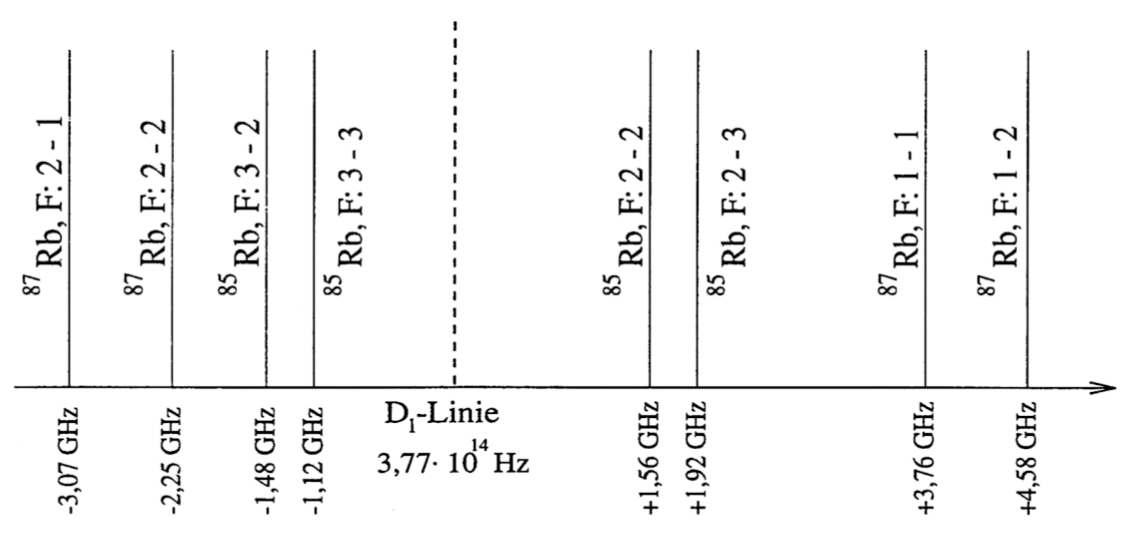
\includegraphics[width=0.7\textwidth]{../img/HFSspect_theo.png}
  \caption{Spektrallinien der Hyperfeinstruktur des ${}^2\text{S}_{1/2}$\,-\,${}^2\text{P}_{1/2}$\,-\,Übergangs
  von \rb{85} und \rb{87} (aus \cite{manual}).}
  \label{img:hfsspectrum}
\end{center}
\end{figure} 

Des Weiteren ist jedes Hyperfeinstrukturniveau $(2F+1)$-fach entartet. Die zugehörige Magnetquantenzahl lautet $m_F$ mit $-F \leq m_F \leq F$. 
Wird ein äußeres Magnetfeld $\vec{B}_0$ ($g_J \mu_B B_0 \ll A$) angelegt, so hebt sich die Entartung auf und es entsteht eine weitere 
Aufspaltung, die \emph{Zeeman}-Aufspaltung der Hyperfeinstruktur.
Für die Energiedifferenz benachbarter Niveaus gilt 
\begin{equation}
    \label{eq:nuclearspin}
    \Delta E_\text{HFS}^\text{Zeeman}(\Delta m_F = 1) = \frac{g_J}{2 \left( I + \frac{1}{2} \right) } \mu_B B_0 \ \, .
\end{equation}
Dabei ist $g_J$ der \emph{Landé-Faktor.}\\
Die Hyperfein- und Zeeman-Aufspaltungen von \rb{85} und \rb{87} sind in \autoref{img:termschema} dargestellt.

\begin{figure}[H]
    \centering
    \def\svgwidth{0.85\textwidth}
    \input{../img/termschema.pdf_tex}
    \caption{Termschemata der beiden Rubidiumisotope:
    Feinstruktur, Hyperfeinstruktur und Zeeman-Aufspaltung der D$_1$-Linie im äußeren Magnetfeld.}
    \label{img:termschema}
\end{figure}

\subsection{Optisches Pumpen}
Die erlaubten Übergänge zwischen elektronischen Energieniveaus bei Absorption von Photonen
werden von den folgenden Auswahlregeln beschrieben:
\begin{equation}
\begin{split}
  & \Delta F = 0, \ \pm 1 \qquad (F = 0 \leftrightarrow F = 0 \text{ ist verboten}) \\
  & \Delta \text{m}_\text{F} = 0, \ \pm 1
  \end{split}
\end{equation}
Wenn das Pumpen nur mit \textsigma$^+$-Licht erfolgt,
dann gilt für jeden induzierten Übergang \mbox{$\Delta \text{m}_\text{F} = +1$}.
Beim Zurückfallen des Elektrons auf das untere Niveau kann sich die Mag\-net\-quan\-ten\-zahl
wieder um $\pm$1 ändern oder konstant bleiben.

Dies führt bei \rb{87} nach längerem Pumpen dazu, dass sich fast alle Atome im Zustand
F=2,\,$\text{m}_\text{F}$=2 des \mbox{${}^2\text{S}_{1/2}$-Niveaus} befinden,
da dies das einzige Niveau ist, von dem aus kein Pumpen mit \textsigma$^+$-Licht möglich ist.
\autoref{img:gr:optpump} zeigt diese Situation.

Für \rb{85} folgt analog, dass in den Zustand ${}^2\text{S}_{1/2}$, F=3,\,$\text{m}_\text{F}$=3 gepumpt wird. 


\begin{figure}[H]
\begin{center}
  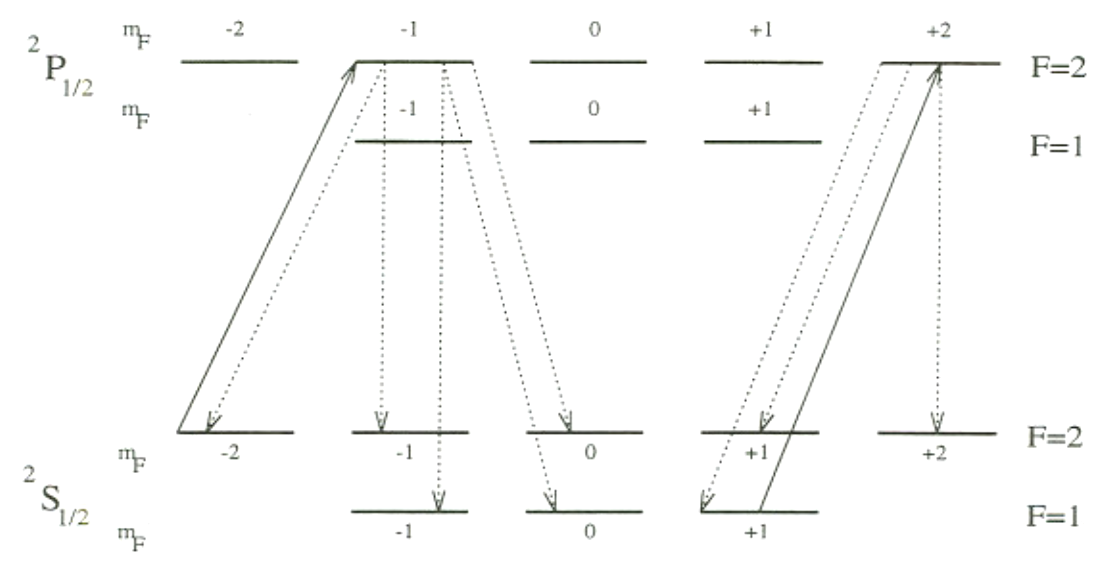
\includegraphics[width=0.85\textwidth]{../img/optPumpen.png}
  \caption{Beispiele für angeregte Übergänge (durchgezogene Linien) beim optischen Pumpen des ${}^2\text{S}_{1/2}$\,-\,${}^2\text{P}_{1/2}$\,-\,Übergangs
  von \rb{87} mit \textsigma$^+$-Licht (aus \cite{staatsex}).
  Die gestrichelten Linien zeigen mögliche Übergänge spontaner Emission.}
  \label{img:gr:optpump}
\end{center}
\end{figure} 

\subsection{Spinpräzession des Rubidiumensembles im äußeren Magnetfeld}
Der Mechanismus der Spinpräzession wird in einem Versuchsteil ausgenutzt,
um die Stärke eines Magnetfelds sehr genau zu bestimmen.
Spinpräzession tritt auf, wenn ein Ensemble von Atomen im Magnetfeld optisch gepumpt,
das Ensemble also polarisiert wird, und anschließend eine Komponente
des Magnetfelds schnell abgeschaltet wird (im Experiment die Komponente in Strahlrichtung).
Die Spins der Atome führen dann eine Präzessionsbewegung um das verbleibende Magnetfeld $\vec{B}$ aus,
im Experiment ist das die Vertikalkomponente.
Die Präzessionsfrequenz $f$ beträgt \cite{staatsex}
\begin{equation}
    \label{eq:gr:spinpräz}
    f=\frac{g_\text{F} \cdot \mu_\text{B}}{h} \cdot B=: \alpha \cdot B
\end{equation}
Hier sind $\mu_\text{B}$ das Bohrsche Magneton, $h$ das Plancksche Wirkungsquantum und
$g_\text{F}$ der Landé-Faktor des Isotops.
Man erhält mit $g_\text{F}$(\rb{85})=1/3 und $g_\text{F}$(\rb{87})=1/2 \cite{staatsex} für
die Proportionalitätskonstante $\alpha$ die Werte
\begin{equation}
    \label{eq:gr:alpha}
    \alpha_{85}=4.665\,\text{kHz } \text{\textmu T}^{-1} \qquad \text{und} \qquad	\alpha_{87}=6.998\,\text{kHz } \text{\textmu T}^{-1} \ \, .
\end{equation}

\subsection{Orientierungsprozesse im Rubidiumensemble}
In diesem Abschnitt wird ein kurzer Überblick über die mathematische Beschreibung der Orientierungsprozesse
(Polarisation und Relaxation) im Rubidiumgas gegeben und es werden die Zusammenhänge aufgeführt, die für die
Auswertung der Messungen zur Relaxationszeit notwendig sind.
Die ausführliche Herleitung der Formeln wird in \cite{staatsex} gezeigt.

Betrachtet man ein Ensemble von Rubidiumatomen, das im Magnetfeld durch zirkular polarisiertes Licht gepumpt wird,
wird die Zunahme der Differenz der Besetzungszahlen~$\left(\frac{\difd n}{\difd t}\right)_{\text{Pump}}$
durch die folgende Differenzialgleichung beschrieben:
\begin{equation}
    \left(\frac{\difd n}{\difd t}\right)_{\text{Pump}}=\frac{N-n}{T_\text{P}}
\end{equation}
$N$ ist die Anzahl der Atome im Ensemble, $n$ die Differenz der Besetzungszahlen in dem Zweiniveausystem
und $T_\text{P}$ die charakteristische Zeit für den Pumpvorgang, die \emph{Pumpzeit}.

Relaxation, also Verlust der Polarisation, ist durch verschiedene Mechanismen möglich:
Durch Wechselwirkung der Atome mit der Wand der Messzelle, durch Stöße mit dem Puffergas
oder durch Spinaustausch zwischen den Rubidiumatomen.
Der Relaxationsvorgang wird durch folgende Differenzialgleichung beschrieben:
\begin{equation}
    \left(\frac{\difd n}{\difd t}\right)_{\text{Relax}}=-\frac{n}{T_\text{R}}
\end{equation}
$T_\text{R}$ ist die \emph{Relaxationszeit}. Der theoretische Wert \cite{staatsex} der Relaxationszeit für die bei der Messung 
verwendete Rubidiumzelle beträgt ohne Berücksichtigung des Spinaustausches
\begin{equation}
    \label{eq:tr:theo}
    T_\text{R}^\text{theo} = 6.5\,\text{ms} \ \, .
\end{equation}

Die Summe von Polarisation und Relaxation beschreibt den Orientierungsprozess im Rubidiumgas mit
der Orientierungszeit $\tau$:
\begin{equation}
    \label{eq:orientierungszeit}
    \left(\frac{\difd n}{\difd t}\right)_{\text{Orient}}
    =\left(\frac{\difd n}{\difd t}\right)_{\text{Pump}} + \left(\frac{\difd n}{\difd t}\right)_{\text{Relax}}
    =\frac{N}{T_\text{P}}-n \left( \frac{1}{T_\text{P}} + \frac{1}{T_\text{R}}\right)
    =:\frac{N}{T_\text{P}}- \frac{n}{\tau}
\end{equation}

Die Lösung dieser Differenzialgleichung für $n(t)$ ist eine exponentielle Änderung mit der Zeitkonstante $\tau$:
\begin{equation}
    \label{eq:expabhorient}
    n(t) \sim e^{-\frac{t}{\tau}}
\end{equation}


\subsection{Die Laserdiode}
Zum optischen Pumpen wird im Versuch eine Laserdiode verwendet,
weil Laserdioden linear polarisiertes Licht in einem schmalen Wellenlängenbereich liefern.
Durch den Laserstrom und die Lasertemperatur kann die Wellenlänge des Lasers gezielt
beeinflusst werden, so dass selektiv einzelne Hyperfein-Übergänge angeregt werden können.
Für den Betrieb des Lasers ist ein Minimalstrom notwendig (die \emph{Laserschwelle}).
Wird dieser Strom überschritten, ändern sich Ausgangsleistung und Laserfrequenz
in erster Näherung linear mit dem Laserstrom.
Es treten allerdings bei der Durchstimmung immer wieder Modensprünge auf,
wenn sich die Zahl der stehenden Wellen im Resonator ändert. Dies äußert sich sowohl in Stufen in der $P$-$I$-Kennlinie 
als auch in unterschiedlich großen Abständen im Spektrum eines Etalons (Funktionsweise siehe \autoref{sub:etalon}).
Bei den Messungen muss darauf geachtet werden, dass keine Modensprünge auftreten,
um eine lineare Durchstimmung des Lasers zu erzielen.

\subsection{Das Fabry-Pérot-Interferometer}
\label{sub:etalon}
Ein Fabry-Pérot-Interferometer (Etalon) besteht aus zwei halbtransparenten, reflektierenden Flächen
im Strahlengang.
Eine Lichtwelle kann transmittiert werden, wenn sie zwischen den Spiegeln konstruktiv mit sich selbst interferiert.
Über die Bedingung für konstruktive Interferenz kann man den \emph{freien Spektralbereich} berechnen,
der den Abstand zwischen zwei Transmissionsmaxima beschreibt.
